\subsection{Nodes and Edges} \label{subsec:nodes_and_edges}
As we progress in our analysis, we now turn our attention to constructing the fundamental building blocks of our network.

First we create a basic PPI network with proteins as nodes and their interactions as edges.
Then we extend the network with genes as nodes that are translated into proteins.
The edges between them are called connections as shown in~\cref{fig:03_02_Network}.

In summary the graph database will consist of four components: genes, proteins,
gene-protein edges (connections), and protein-protein edges (interactions).
For each of these components, we create a table with their necessary attributes.

% Cypher Query für Bild:
% MATCH (g:gene) WITH g LIMIT 4
% MATCH (g)-[r1]-(p:protein) WITH g, p, r1 LIMIT 20
% OPTIONAL MATCH (p)-[r2]-()
% RETURN g, collect(r1) AS gene_edges, p, collect(r2) AS protein_edges LIMIT 50

\begin{figure}[!h]
    \centering
    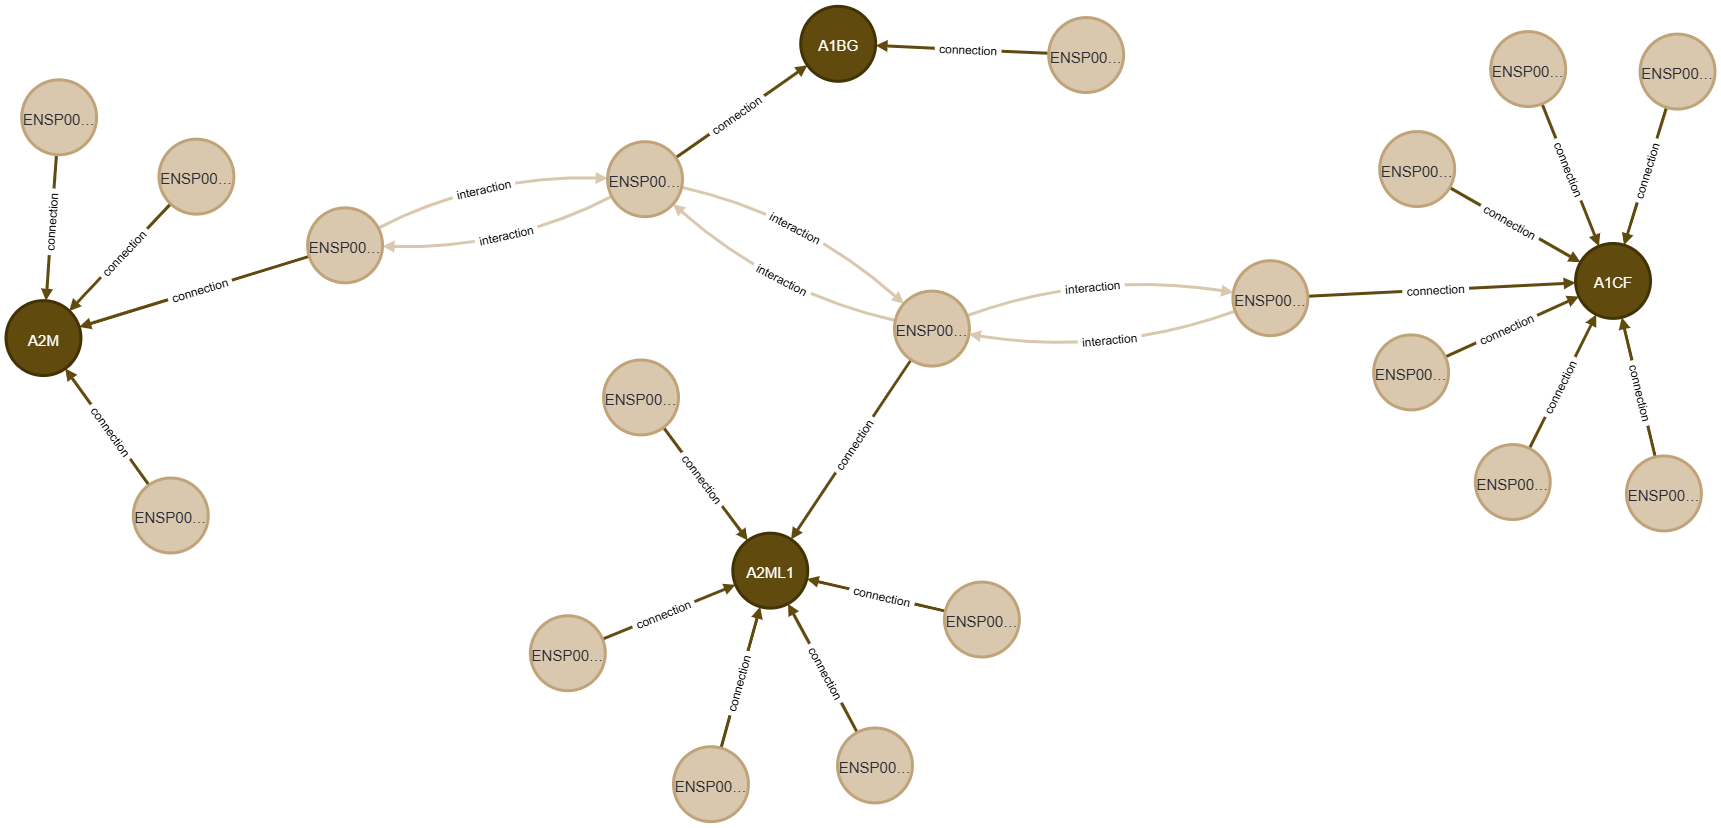
\includegraphics[width=1\textwidth]{figures/03_02_Network_2}
    \caption{Extract from the graph database setup with genes in dark brown and proteins in light brown including their edges}
    \label{fig:03_02_Network}
\end{figure}

% Structure:
%   Protein-Protein Edges
%   Gene-Protein Edges
%   Gene Nodes
%   Protein Nodes


%%%%%%%%%%%%%%%%%%%%%%%%%%%%%%%%%%%%%%%%%%%%%%%%%%%%%%%%%%%%%%%%%%%%%%%%%%%%%%%%%%%%%%%%%%%%%%%%%%%%%%%%%
% NUMBERS CHECKED!!!
\subsubsection*{Protein-protein edges} \label{subsubsec:protein_protein_edges}
To create the protein-protein edges we use the data from the String (Search Tool for the Retrieval of Interacting Genes/Proteins) Database.
This database is a comprehensive resource for studying protein-protein interactions and often used in research~\cite{Szklarczyk2020String}.
The protein links file for Homo sapiens, which we download from the database website~\cite{string_download},
contains 13,715,404 rows of protein-protein edges (\cref{fig:03_02_df_protein_edges}).
Each row includes two protein IDs, representing the edge between them.

Since no additional attributes are required for this table, we do not need to perform any further editing.

\begin{figure}[h]
    \centering
    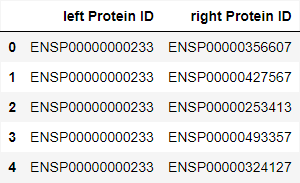
\includegraphics[height=\dfheight]{figures/03_02_protein_edges}
    \caption{Example data of protein-protein edges that will be used as interaction between proteins in the graph database}
    \label{fig:03_02_df_protein_edges}
\end{figure}



%%%%%%%%%%%%%%%%%%%%%%%%%%%%%%%%%%%%%%%%%%%%%%%%%%%%%%%%%%%%%%%%%%%%%%%%%%%%%%%%%%%%%%%%%%%%%%%%%%%%%%%%%
% NUMBERS CHECKED!!!
\subsubsection*{Gene-protein edges} \label{subsubsec:gene_protein_interaction}
To build the connections between genes and proteins, we need to link each gene to its corresponding protein translation.
For this purpose, we downloaded a file from biomart containing Gene IDs and their Protein IDs for the human genome~\cite{bio_marts}
The initial dataset comprised of 185,330 entries.

First we drop any rows where either the Ensembl ID for gene or protein is missing, as these would represent incomplete edges.
Next we built the intersection of rows where the gene ID matched an existing gene node (as described in \ref{subsubsec:gene_nodes}~-~Gene nodes)

The final gene-protein edge table~(\cref{fig:03_02_df_gene_protein_edges}) features 101,731 rows as edges and two columns:
Ensembl ID for the gene and Ensembl ID for the protein.

\begin{figure}[h]
    \centering
    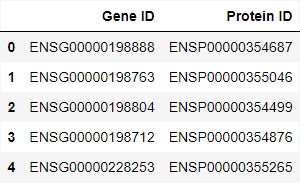
\includegraphics[height=\dfheight]{figures/03_02_gene_protein_edges}
    \caption{Example data of gene-protein edges that will be used as connection between genes and proteins in the graph database}
    \label{fig:03_02_df_gene_protein_edges}
\end{figure}



%%%%%%%%%%%%%%%%%%%%%%%%%%%%%%%%%%%%%%%%%%%%%%%%%%%%%%%%%%%%%%%%%%%%%%%%%%%%%%%%%%%%%%%%%%%%%%%%%%%%%%%%%
% NUMBERS CHECKED!!!
\subsubsection*{Gene nodes} \label{subsubsec:gene_nodes}

To create the rows for our table of gene nodes, we use the preprocessed CMP and GTEx datasets,
which contain mean TPM values for cancerous and healthy genes.
We build the intersection of both datasets on their gene Ensemble ID to get a subset.
The new dataset only contains genes with TPM values for both conditions.

% TODO Code - put code for gene-protein to gene file?!
Next we want to filter for genes that are translated into proteins.
Because other types of genes would have no connection to the protein nodes in the network.
Therefor we build a new subset of genes that also occur in the gene-protein edge table (\ref{subsubsec:gene_protein_interaction}~-~Gene-protein edges).

Now we have all rows we need for our gene nodes, and we want to focus on the columns that we will need as attributes.
When examining the mean TPM values per dataset, we observe a right-skewed distribution, with most values close to zero
and a long tail extending towards higher values.
The cancerous TPM values vary from 0 to approximately 41,173 and the healthy TPM values range from 0 to around 36,200.

To fulfill our first objective~\ref{obj:delta_tpm} for these genes,
we want to calculate a measure that captures significant changes between cancerous and healthy gene activity.
First we normalize the TPM values from both datasets by performing a common log scaling between 0 and 1 for all TPM values.

\begin{equation}
\label{eq:tpm_normalization}
log\_norm(x) = \frac{\log(1 + x) - \log(1 + x_{min})}{\log(1 + x_{max}) - \log(1 + x_{min})}
\end{equation}

where $x_{\max}$ and $x_{\min}$ are the maximum and minimum TPM values across both datasets.
After applying the normalization, the distribution of the TPM values is more balanced, as shown in \cref{fig:03_02_normalized_tpm_both}.

\begin{figure}[h]
\minipage{0.45\textwidth}
    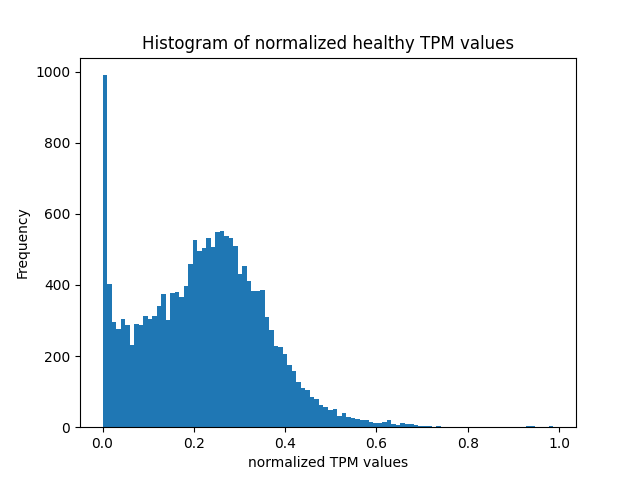
\includegraphics[width=\linewidth]{figures/03_02_normalized_gtex_tpm}
\endminipage
\hfill
\minipage{0.45\textwidth}
  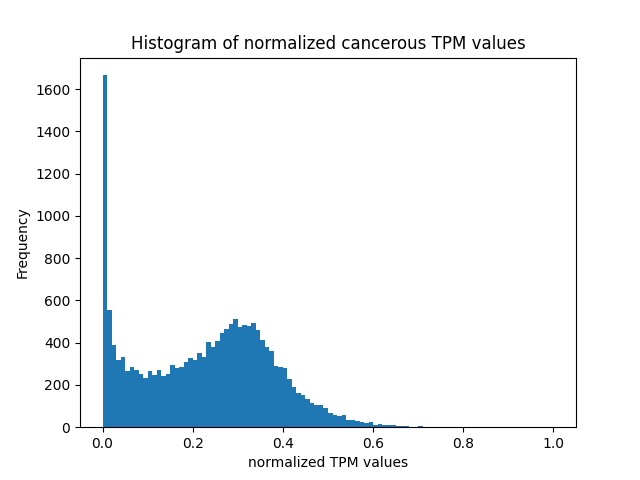
\includegraphics[width=\linewidth]{figures/03_02_normalized_cmp_tpm}
\endminipage
\caption{Normalized mean healthy and cancerous TPM values between 0 and 1}
\label{fig:03_02_normalized_tpm_both}
\end{figure}


Next, we calculate the difference between the normalized mean healthy and cancerous TPM values per gene
by subtracting the two values and call it $\Delta_{TPM}$.
The distribution of $\Delta_{TPM}$ values is shown in \cref{fig:03_02_delta_tpm}.

\begin{figure}[h]
    \centering
    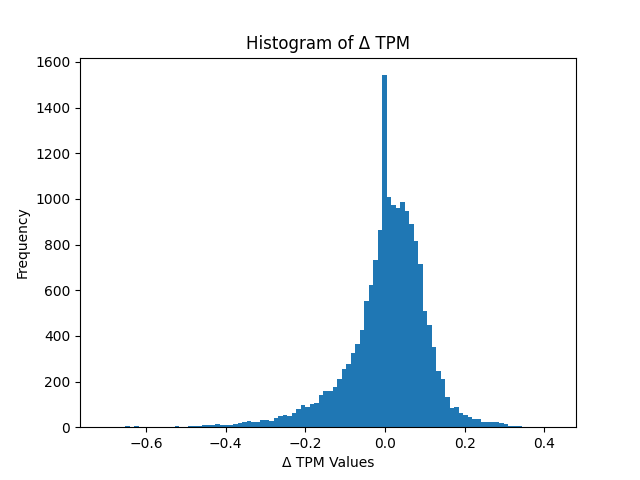
\includegraphics[width=0.5\textwidth]{figures/03_02_delta_tpm}
    \caption{Distribution of the difference between the normalized mean healthy and cancerous TPM values, called $\Delta_{TPM}$ values}
    \label{fig:03_02_delta_tpm}
\end{figure}

We then define an $\Delta_{type}$ as either $increase$ or $decrease$, depending on whether the delta value is positive or negative.

As the final step for the objective, we need to determine if a change in gene activity is relevant.
To do this, we use the z score measure, which calculates how many standard deviations a $\Delta_{TPM}$ value is away
from the mean of all $\Delta_{TPM}$ values.
The $z score$ is given by:

\begin{subequations}
    \begin{equation} \label{eq:z_score}
        z score (x) = \frac{x - {\mu}}{\sigma}
    \end{equation}
    \begin{equation}
        \text{where } \mu = \frac{1}{n} \sum_{i=1}^{n} x_i
        \label{eq:mean}
    \end{equation}
    \begin{equation}
        \text{where } \sigma = \sqrt{\frac{1}{n} \sum_{i=1}^{n} (x_i - \mu)^2}
        \label{eq:std}
    \end{equation}
\end{subequations}

where $x$ is the $\Delta_{TPM}$ value, $\mu$ is the mean of all $\Delta_{TPM}$ values, $\sigma$ is the standard deviation of all $\Delta_{TPM}$ values.

We define a threshold of $z score = 1.96$ to indicate significant changes in gene activity,
which corresponds to a confidence level of 95\% (p = 0.05).
Genes with $\Delta_{TPM}$ values exceeding this threshold will be flagged as $true$ in the $\Delta_{TPM\_relevant}$ column.
By this we fulfilled our first objective~\ref{obj:delta_tpm} by finding 1,034 genes with significant changes in gene activity.

The resulting table contains 17,627 gene nodes as rows with their associated attributes,
including TPM values and derived metrics such as $\Delta_{TPM}$ or $z score$.
The head of the table is shown in~\cref{fig:03_02_df_gene_nodes}.

\begin{figure}[h]
    \centering
    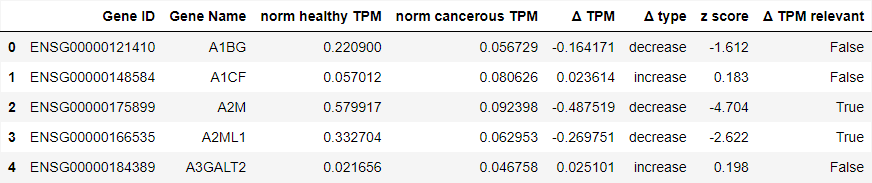
\includegraphics[height=\dfheight]{figures/03_02_gene_nodes}
    \caption{Example data of gene nodes that will be used in the graph database}
    \label{fig:03_02_df_gene_nodes}
\end{figure}




%%%%%%%%%%%%%%%%%%%%%%%%%%%%%%%%%%%%%%%%%%%%%%%%%%%%%%%%%%%%%%%%%%%%%%%%%%%%%%%%%%%%%%%%%%%%%%%%%%%%%%%%%
% NUMBERS CHECKED!!!
\subsubsection*{Protein nodes} \label{subsubsec:protein_nodes}
Lastly we create the table for the protein nodes.
To collect all protein nodes for our database creation we use the gene-protein edges(\cref{subsubsec:gene_protein_interaction}~-~Gene-protein edges)
and the protein-protein edges (\ref{subsubsec:protein_protein_edges}~-~Protein-protein-edges), which we already created.

From the gene-protein edge table, we extract all unique protein Ensembl IDs.
From the protein-protein edge table, we concat both columns of protein Ensembl IDs and extract all unique values.
We then merge both tables and drop duplicates again to get a list of all unique protein Ensembl IDs from both tables.

The resulting table is a list of 104,235 unique Protein Ensembl IDs as shown in \cref{fig:03_02_df_protein_nodes}.

\begin{figure}[h]
    \centering
    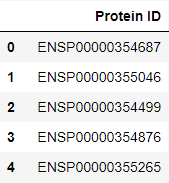
\includegraphics[height=\dfheight]{figures/03_02_protein_nodes}
    \caption{Example data of protein nodes that will be used in the graph database}
    \label{fig:03_02_df_protein_nodes}
\end{figure}


% TODO Protein Nodes is single column - can library also save this?